% Trabajo de estudiante en formato APA 7.a edicion (espanol).
% Compilar con XeLaTeX: xelatex aplicacion-medicontrol.tex
\documentclass[stu,letterpaper,floatsintext,nolmodern,nofontenc]{apa7}

\usepackage{fontspec}
\setmainfont{Times New Roman}
\usepackage[spanish,es-noshorthands]{babel}
\usepackage{csquotes}
\usepackage{indentfirst}
\usepackage{etoolbox}

% APA 7 no usa guiones automaticos al final de la linea.
\hyphenpenalty=10000
\exhyphenpenalty=10000

% El escudo institucional va en la portada, encima del titulo.
\makeatletter
\patchcmd{\maketitle}{\vspace*{4\baselineskip}}{%
  
\includegraphics[width=2.45cm]{figuras/logo-unifranz.png}\\[0.6\baselineskip]
}{}{%
  \PackageWarning{medicontrol}{No se pudo insertar el logo en la portada}%
}
\makeatother

\title{Aplicación Móvil para Gestión de Pacientes y Citas}
\authorsnames{Miguel Angel Andrade Arnez}
\authorsaffiliations{Universidad Franz Tamayo, Facultad de Ingeniería, Carrera de Ingeniería de Sistemas}
\course{Sistemas Operativos Móviles y Embebidos}
\professor{Ing. Christian Luis Lopez Bravo}
\duedate{8 de septiembre de 2026}

\begin{document}
\maketitle

\subsection{Descripción de las Funcionalidades de la Aplicación MediControl}

MediControl será una aplicación móvil orientada a facilitar la gestión de pacientes, consultas y citas médicas dentro de una clínica. El sistema permitirá organizar la información de manera digital, reduciendo el uso de registros manuales y facilitando el acceso rápido a la información.

\subsection{Inicio de Sesión}

Esta opción permitirá que el personal autorizado de la clínica ingrese a la aplicación mediante un correo electrónico y una contraseña. El objetivo es proteger la información de los pacientes y evitar que personas no autorizadas puedan acceder a los datos médicos.

Una vez que el usuario haya ingresado correctamente sus credenciales, podrá acceder a las diferentes funciones disponibles dentro de la aplicación.

\subsection{Pantalla Principal}

La pantalla principal funcionará como el panel de inicio de la aplicación. Desde aquí el usuario podrá acceder rápidamente a las principales funciones del sistema, como pacientes, citas, historial médico y tratamientos.

También mostrará información importante, como la próxima cita programada, permitiendo al personal de la clínica tener una visión rápida de las actividades pendientes.

\subsection{Lista de Pacientes}

Esta opción permitirá registrar, buscar y consultar los pacientes de la clínica. El usuario podrá visualizar información básica como el nombre del paciente, número de identificación y fecha de su última consulta.

Además, contará con una opción de búsqueda para encontrar rápidamente a un paciente sin necesidad de revisar manualmente todos los registros.

\subsection{Perfil del Paciente}

Al seleccionar un paciente, la aplicación mostrará su información detallada. En esta sección se podrán consultar datos personales, información de contacto, historial de consultas y tratamientos registrados.

El objetivo es que el personal médico pueda acceder rápidamente a los antecedentes del paciente antes o durante una consulta, manteniendo toda la información organizada en un solo lugar.

\subsection{Agenda de Citas}

La agenda permitirá visualizar las citas médicas programadas mediante un calendario. El usuario podrá consultar las citas correspondientes a cada día y conocer la hora, paciente y motivo de la consulta.

Esta función ayudará a organizar mejor la atención de la clínica y permitirá reducir problemas relacionados con el manejo manual de las citas.

\subsection{Nueva Cita}

Esta opción permitirá registrar una nueva cita médica. El usuario podrá seleccionar al paciente, establecer la fecha y hora de la consulta e indicar el motivo de la atención.

Una vez guardada, la cita aparecerá automáticamente en la agenda de la aplicación para que pueda ser consultada posteriormente.

\subsection{Funciones Adicionales}

Como parte de futuras versiones del sistema, MediControl podrá incorporar funciones adicionales como recordatorios de citas, gestión de recetas y tratamientos, sincronización de información y mecanismos de seguridad para proteger los datos almacenados.

Estas funciones permitirán que la aplicación pueda crecer progresivamente y adaptarse a las necesidades de la clínica.

\section{Objetivo General de la Aplicación}

El objetivo de MediControl es digitalizar y organizar la gestión de pacientes y citas médicas de una clínica mediante una aplicación móvil, permitiendo acceder a la información de forma rápida, ordenada y segura.

La aplicación busca mejorar el control de la información, facilitar el trabajo del personal de la clínica y reducir la dependencia de registros realizados manualmente. En la Figura 1 se muestran las pantallas de inicio de sesión, pantalla principal, lista de pacientes, perfil del paciente, agenda de citas y registro de una nueva cita.

\begin{figure}
\caption{Pantallas de MediControl para el inicio de sesión, la pantalla principal, la lista de pacientes, el perfil del paciente, la agenda de citas y el registro de una nueva cita}
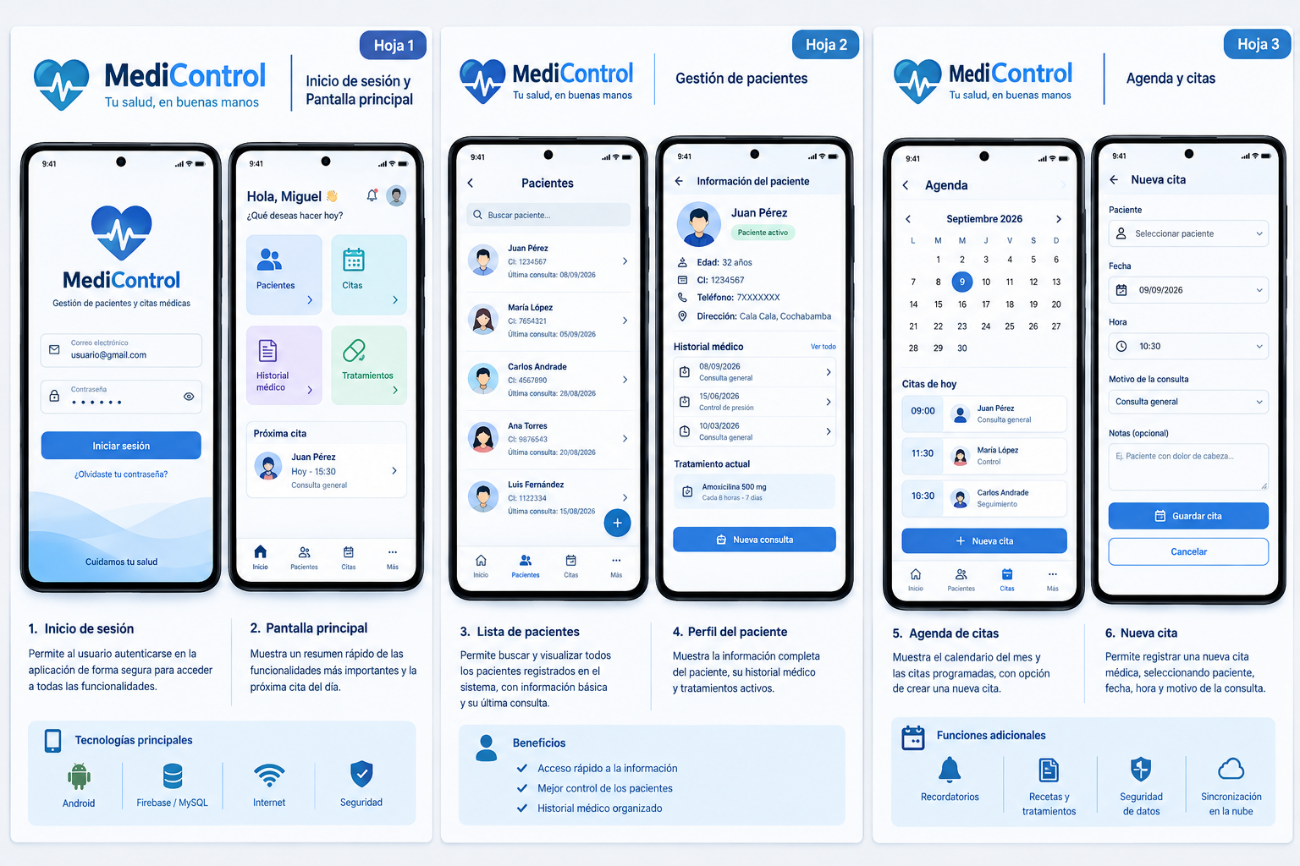
\includegraphics[width=\linewidth]{figuras/interfaz-medicontrol.png}
\end{figure}

\end{document}
